

%preamble

\documentclass[english]{article}
\usepackage{fullpage}
\usepackage[T1]{fontenc}
\usepackage[latin9]{inputenc}
\setlength{\parskip}{\medskipamount}
\setlength{\parindent}{0pt}

\usepackage{amsmath}
\usepackage{amssymb}
\usepackage{amsthm}
\usepackage{amsfonts}
\usepackage{graphicx}
\usepackage[all,arc,curve,frame]{xy}

\newcommand{\Nat}{\mathbb{N}}
\newcommand{\defeq}{:=}
\newcommand{\vect}[1]{\boldsymbol{#1}}

\renewcommand{\labelenumii}{\arabic{enumi}.\arabic{enumii}.}
\renewcommand{\labelenumiii}{\arabic{enumi}.\arabic{enumii}.\arabic{enumiii}.}
\renewcommand{\labelenumiv}{\arabic{enumi}.\arabic{enumii}.\arabic{enumiii}.\arabic{enumiv}.}



\usepackage{tikz}
\usetikzlibrary{arrows}
\usepackage{listings}


\begin{document}
\title{
 CS5811 In-Progress Report:\\
 Search for Self-Stabilizing Protocols
}

\author{~Brandon~Crowley,~Alex~Klinkhamer, and~Mandy~Wang}
\maketitle



%{\it Formulate the search problem: states, actions, goals.}

\section{Progress}

\begin{itemize}
 \item We investigated how to represent state predicates and actions with MDDs.
  This is explained below and we have prototype code for it.
 \item We have also figured out how to perform forward and backwards reachability using MDDs, though this is not explained in the report yet.
  As a corollary, this means we know how to check for weak stabilization using MDDs.
 \item At the end of this report (in the last example), we show the input file format we may use.
  In that example, we also show how a generated protocol would look.
\end{itemize}

\section{Future Work}

Our current to-do list consists primarily of constructing a detailed list of activities required to finish this project, with a rough timeline 
and initial task assignments for each member, all of which will be taken care of early in the next week, and then we will begin with whichever tasks top
the new list.  After that, our broader to-do list consists of the items laid out in section 2 of the proposal, less items already completed:
cycle checking, weak stabilization checking, the backtracking algorithm, implementing the most-constrained variable and AC-3 heuristics, and performing
tests to measure the effectiveness of our implementation.

\section{BDD Algorithms}
As in regular software or any search algorithm, the states could be of large amount and rather complex. Simply listing the states is inefficient and complicates analysis. Here we resort to Multiple-Valued Logic for describing the state of a system, represented by a multiple-valued decision diagram (MDD), which is general version of BDD. This allows countermeasures to be formated that address states that share common features. 

Both BDDs and MDDs represent expressions connected by disjunctions and conjunctions to form a state predicate and output true or false. The difference between BDD and MDD is that BDD only permit boolean values assigned to each variable while MDD assigns numbers within an indicated domain to the variables as state predicate. MDD has been developed and implemented to construct BDD. 

Consider a predicate over three variables $x, y, z$, each with values ranging from $0$ to $4$ (domain size 3). Initially, there are $5^3 = 125$ states in the system. If we specify the state predicate as $x=3$, the number of states for which the predicate returns {\it true} is $25$, since the value of $x$ is totally fixed. We could use an MDD to symbolically represent this set of $25$ states.

Now we have a rough format close to the format representing the protocol states later on. Say there are 3 processes arranged in the bidirectional ring, and each node could read from its two neighbors and write to itself. Actually, with three processes in a bidirectional ring, each process can read all variables, but the small state-space is convenient for this example. We use $m_0$ as the variable of $P_0$. $m'_0$ means the same except the value is the one in the next time step. Similarly, this rule applies to processes $P_1$ and $P_2$. The following predicate represents a transition function for this system:
\begin{eqnarray*}
 & & m_0 = 0 \wedge m'_0 = 0 \wedge m_1 = 0 \wedge m'_1 = 1 \wedge m_2 = 1 \wedge m'_2 = 1 \\
 & \vee & m_0 = 0 \wedge m'_0 = 0 \wedge m_1 = 2 \wedge m'_1 = 1 \wedge m_2 = 1 \wedge m'_2 = 1
\end{eqnarray*}
After checking the values of each process, it is obvious that there are some variables which will change their values as time goes on. The value of $m_1$ can change to $1$ from $0$ when $m_0 = 0 \wedge m_1 = 0 \wedge m_2 = 1$. The value of $m_1$ can also change to $1$ from $2$ when $m_0 = 0 \wedge m_1 = 2 \wedge m_2$. This shows how to represent a transition function with satisfying valuations of unprimed and primed variables.

%In another aspect, a formula could be created as the evaluation standard for judging whether a state is a legitimate state or not. Still in the above instance, if $(m_0={m'}_0)\cap (m_2={m'}_2)\cap (m_0=0)\cap (m_2=1)\cap (m_1=0\cup m_1=2)\cap ({m'}_1=1)$ is the standard for telling whether the questioned state is an illegitimate state, then the two states above are illegitimate states since the output from the standard is true. Therefore, an action is required, which could be ${m'}_1=1$, to transfer the state into legitimate state region, and therefore stabilize the system.

\section{Examples}
Some examples of stabilizing protocols follow.
We plan to use these (and more) in our experimentation.

We should also try to use reduction to SAT on these problems, but encoding cycle detection in a CNF formula blows up quickly in size.
In the worst case, we require $O(\abs{S_p}^3)$ where $S_p$ is set of all states.
Our tool should outperform the reduction to SAT purely due to its exploding size.

\subsection{Dijkstra's Token Ring}
Let us consider the original token ring protocol Dijkstra used when introducing the concept of self-stabilization \cite{dij}.
A token ring is used to give one process out of many an exclusive right, also known as distributed mutual exclusion.
Below is a ring of $n=6$ finite-state machines (processes).

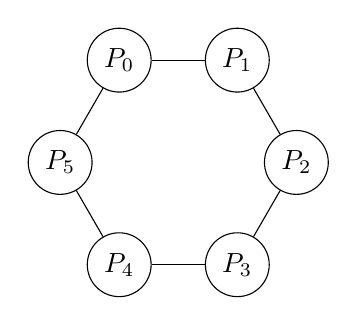
\begin{tikzpicture}[x=1.5cm,y=1.5cm]
 \tikzstyle{every node}=[draw,circle]
 \draw
 (0,0)      node (0) {$P_0$}
 ++(   0:1) node (1) {$P_1$}
 ++( -60:1) node (2) {$P_2$}
 ++(-120:1) node (3) {$P_3$}
 ++(-180:1) node (4) {$P_4$}
 ++(-240:1) node (5) {$P_5$}
 ;
 \draw (0) -- (1);
 \draw (1) -- (2);
 \draw (2) -- (3);
 \draw (3) -- (4);
 \draw (4) -- (5);
 \draw (5) -- (0);
\end{tikzpicture}

Each process $P_i$ holds a variable $x_i$ which ranges from $0$ to $n$ ($x_i\in\Nat_{n+1}$).
Each $P_i$ can read and write $x_i$ and can read $x_{i-1}$ (where subtraction is modulo $n$).
Note that each process can only read its left neighbor, so we call this ring {\em unidirectional}.

$P_0$ is said to have a token when it sees $x_{n-1} = x_0$.
Any other $P_i$ has a token when $x_{i-1} \neq x_i$.

A state is legitimate when exactly one process has the token.

\[
\begin{array}{rrcl}
 P_0: & x_{5} = x_0 & \to & x_0 \defeq x_0 + 1 \mod (n+1)
\\ P_{i>0}: & x_{i-1} \neq x_i & \to & x_i \defeq x_{i-1}
\end{array}
\]

\subsection{Maximal Matching}

Let each process $P_i$ in a bidirectional ring of $n$ processes have a variable $m_i\in \Nat_3$ (i.e., $m_i\in \{0,1,2\}$) where each of the three values represents a different direction, like {\it self} ($m_i=0$), {\it left} ($m_i=1$), and {\it right} ($m_i=2$).
Since this is a bidirectional ring, any $P_i$ can read its left and right neighbors' variables $m_{i-1}$ and $m_{i+1}$.
$P_i$ can also read and write its own variable $m_i$.

The system is in a legitimate state when neighbors pair up by pointing at each other.
If both neighbors are pointing away, a process can point at itself.
Formally, the invariant is defined as (with arithmetic modulo $n$):
\begin{eqnarray*}
 I \equiv \forall i\in\Nat_n: & & (m_{i-1} = 2 \wedge m_i = 1)
                    \\ & \vee  & (m_{i-1} = 1 \wedge m_i = 0 \wedge m_{i+1} = 2)
                    \\ & \vee  & (m_i = 2 \wedge m_{i+1} = 1)
\end{eqnarray*}

\subsection{3-Coloring on a Ring}

Let each process $P_i$ in a bidirectional ring of $n$ processes have a variable $c_i\in \Nat_3$ (i.e., $c_i\in \{0,1,2\}$) where each of the three values represents a different color, like {\it red}, {\it green}, and {\it blue}.
Since this is a bidirectional ring, any $P_i$ can read its left and right neighbors' variables $c_{i-1}$ and $c_{i+1}$.
$P_i$ can also read and write its own variable $c_i$.

The system is in a legitimate state when no two neighboring processes have the same color.
Formally, the invariant is defined as (with arithmetic modulo $n$):
\[ I \equiv (\forall i\in\Nat_n: c_{i-1}\ne c_i \wedge c_i \ne c_{i+1}) \]

The following file expresses this system and invariant using input format of Sycraft \cite{sycraft2008}.

\fbox{
 \lstinputlisting{ThreeColoring.fin}
}

The following action for each $P_i$ can be used for a stabilizing protocol:
\[
 (c_{i-1} = c_i) \vee (c_i = c_{i+1}) \to c_i \defeq \textsc{Other}(c_{i-1}, c_{i+1})
\]
where the \textsc{Other} function returns a color (deterministically, say the minimal-valued one) which is not equal to either of its inputs.

We expect our tool to synthesize actions in their most basic form, as local state transitions.
The above action can be expressed by the following $15$ local state transitions for $P_i$:
\begin{eqnarray*}
 c_{i-1} = 0 \wedge c_i = 0 \wedge c_{i+1} = 0 & \to & c_i \defeq 1 \\
 c_{i-1} = 0 \wedge c_i = 0 \wedge c_{i+1} = 1 & \to & c_i \defeq 2 \\
 c_{i-1} = 1 \wedge c_i = 0 \wedge c_{i+1} = 0 & \to & c_i \defeq 2 \\
 c_{i-1} = 2 \wedge c_i = 0 \wedge c_{i+1} = 0 & \to & c_i \defeq 1 \\
 c_{i-1} = 0 \wedge c_i = 0 \wedge c_{i+1} = 2 & \to & c_i \defeq 1 \\
 c_{i-1} = 1 \wedge c_i = 1 \wedge c_{i+1} = 1 & \to & c_i \defeq 0 \\
 c_{i-1} = 1 \wedge c_i = 1 \wedge c_{i+1} = 0 & \to & c_i \defeq 2 \\
 c_{i-1} = 0 \wedge c_i = 1 \wedge c_{i+1} = 1 & \to & c_i \defeq 2 \\
 c_{i-1} = 1 \wedge c_i = 1 \wedge c_{i+1} = 2 & \to & c_i \defeq 0 \\
 c_{i-1} = 2 \wedge c_i = 1 \wedge c_{i+1} = 1 & \to & c_i \defeq 0 \\
 c_{i-1} = 2 \wedge c_i = 2 \wedge c_{i+1} = 2 & \to & c_i \defeq 0 \\
 c_{i-1} = 2 \wedge c_i = 2 \wedge c_{i+1} = 0 & \to & c_i \defeq 1 \\
 c_{i-1} = 0 \wedge c_i = 2 \wedge c_{i+1} = 2 & \to & c_i \defeq 1 \\
 c_{i-1} = 2 \wedge c_i = 2 \wedge c_{i+1} = 1 & \to & c_i \defeq 0 \\
 c_{i-1} = 1 \wedge c_i = 2 \wedge c_{i+1} = 2 & \to & c_i \defeq 0
\end{eqnarray*}


\bibliographystyle{plain}
\bibliography{bibliography}

\end{document}

